% Preamble: \usepackage{booktabs,tabularx,graphicx,tikz}
%           \usetikzlibrary{positioning,arrows.meta,calc}
\section{Methodology}
\label{sec:method}

%We start from the 731 tasks of the original SWE-Bench Pro Public. A task consists of an instruction (problem statement, requirements, new interfaces), a container image with the repository at its base commit, a reference patch, a hidden test patch, fail-to-pass and pass-to-pass lists naming the graded tests, and a verifier that applies the test patch, runs the tests and parses the output. A task is valid if every solution that satisfies the instruction passes and every solution that does not, fails. Our agentic audits flagged 200 tasks (27\%), and engineers adjudicated each flag (Figure~\ref{fig:pipeline}). The released set has 642 tasks: 531 never flagged, 66 repaired and 45 flagged but kept unchanged. The remaining 89 were discarded.
We start from the 731 tasks of the original SWE-Bench Pro Public. A task consists of an instruction (problem statement, requirements, new interfaces), a container image with the repository at its base commit, a reference patch, a hidden test patch, fail-to-pass and pass-to-pass lists naming the graded tests, and a verifier that applies the test patch, runs the tests and parses the output. A task is valid if every solution that satisfies the instruction passes and every solution that does not, fails. An initial round of repairs addressed test and fixture files leaked into reference patches and instructions that lacked the standard template (40 images). After that, we ran an automated audit, which covers difficulty calibration, instruction–test alignment and reward hacking. Over the total set, 387 tasks were flagged (52\%), with 326 clean and 18 audit errors. Engineers then revised the tasks to align instructions with the graded tests and to improve test coverage of the stated requirements, re-auditing each batch. All 731 tasks were revised, and about 700 passed the automated audit. About 30 could not be made to pass through task edits alone. These were contradictions between base-commit tests and the reference patch, mutation of snapshot or fixture files, and over-flagged or miscalibrated tasks. We also applied three changes to every task. We removed the \textit{"do not edit tests"} constraint from the instruction template and had the verifier revert test-related changes before applying the test patch. We scrubbed git history from the container images so that agents cannot recover the fix from the repository. And we disabled network access in the agent phase, after a frontier model copied reference solutions verbatim from GitHub on 351 solved tasks, only 237 of which held up with GitHub blocked. A second round of fixes was then kicked off focusing on instruction-test alignment, where agentic audits flagged 200 tasks (27\%), and engineers adjudicated each flag (Figure~\ref{fig:pipeline}). The final released V2 set has 642 tasks: 531 never flagged, 66 repaired and 45 flagged but kept unchanged. The remaining 89 were discarded. We discuss each of these stages.
%\jeff{do we describe swe-bench pro v1.1 anywhere? iirc v1.1 already came with significant expert annotation, so we should make it clear that we are starting from a stronger baseline} \jeff{here's what I got from double checking these numbers: Against the v1.1 bundles, the repaired 642 differ in instruction on 161 tasks, and the v2.4 release on 227.} 

%% Pipeline figure for Section~\ref{sec:method}: flow of the 731 tasks.
% Band and bar heights are proportional to task counts (0.046 mm per task).
% Preamble: \usepackage{tikz,graphicx} (xcolor is loaded by tikz)
\definecolor{sbpFlag}{HTML}{4C72B0}
\definecolor{sbpRep}{HTML}{55A868}
\definecolor{sbpDisc}{HTML}{C44E52}
\definecolor{sbpKeep}{HTML}{7F7F7F}
\definecolor{sbpNone}{HTML}{B0B0B0}
\begin{figure*}[t]
\centering
\resizebox{\textwidth}{!}{%
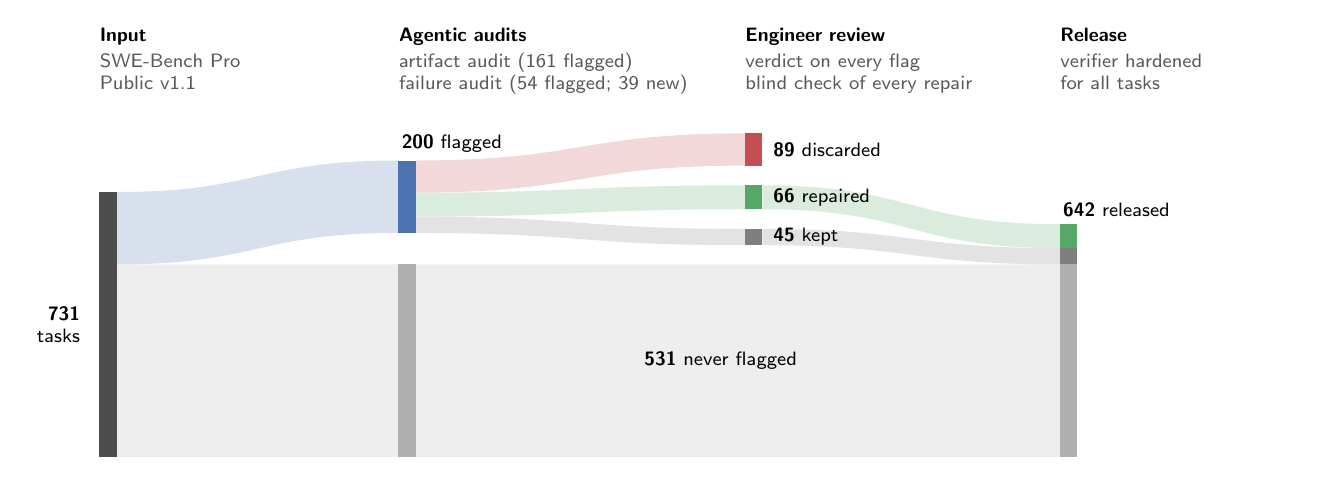
\begin{tikzpicture}[x=1mm, y=1mm, font=\sffamily\scriptsize,
  execute at begin node={\hyphenpenalty=10000\exhyphenpenalty=10000}]
% flagged by an audit
\fill[sbpFlag!22] (2.2,4.09) .. controls (20.1,4.09) and (20.1,8.09) .. (38,8.09)
  -- (38,-1.11) .. controls (20.1,-1.11) and (20.1,-5.11) .. (2.2,-5.11) -- cycle;
% never flagged
\fill[sbpNone!22] (2.2,-5.11) .. controls (20.1,-5.11) and (20.1,-5.11) .. (38,-5.11)
  -- (38,-29.54) .. controls (20.1,-29.54) and (20.1,-29.54) .. (2.2,-29.54) -- cycle;
% discarded
\fill[sbpDisc!22] (40.2,8.09) .. controls (61.1,8.09) and (61.1,11.53) .. (82,11.53)
  -- (82,7.44) .. controls (61.1,7.44) and (61.1,4) .. (40.2,4) -- cycle;
% repaired
\fill[sbpRep!22] (40.2,4) .. controls (61.1,4) and (61.1,4.94) .. (82,4.94)
  -- (82,1.9) .. controls (61.1,1.9) and (61.1,0.96) .. (40.2,0.96) -- cycle;
% kept unchanged
\fill[sbpKeep!22] (40.2,0.96) .. controls (61.1,0.96) and (61.1,-0.6) .. (82,-0.6)
  -- (82,-2.67) .. controls (61.1,-2.67) and (61.1,-1.11) .. (40.2,-1.11) -- cycle;
% never flagged, passes review
\fill[sbpNone!22] (40.2,-5.11) .. controls (81.1,-5.11) and (81.1,-5.11) .. (122,-5.11)
  -- (122,-29.54) .. controls (81.1,-29.54) and (81.1,-29.54) .. (40.2,-29.54) -- cycle;
% repaired -> release
\fill[sbpRep!22] (84.2,4.94) .. controls (103.1,4.94) and (103.1,0) .. (122,0)
  -- (122,-3.04) .. controls (103.1,-3.04) and (103.1,1.9) .. (84.2,1.9) -- cycle;
% kept -> release
\fill[sbpKeep!22] (84.2,-0.6) .. controls (103.1,-0.6) and (103.1,-3.04) .. (122,-3.04)
  -- (122,-5.11) .. controls (103.1,-5.11) and (103.1,-2.67) .. (84.2,-2.67) -- cycle;
% nodes
\fill[black!70] (0,-29.54) rectangle (2.2,4.09);
\fill[sbpFlag] (38,-1.11) rectangle (40.2,8.09);
\fill[sbpNone] (38,-29.54) rectangle (40.2,-5.11);
\fill[sbpDisc] (82,7.44) rectangle (84.2,11.53);
\fill[sbpRep] (82,1.9) rectangle (84.2,4.94);
\fill[sbpKeep] (82,-2.67) rectangle (84.2,-0.6);
\fill[sbpRep] (122,-3.04) rectangle (124.2,0);
\fill[sbpKeep] (122,-5.11) rectangle (124.2,-3.04);
\fill[sbpNone] (122,-29.54) rectangle (124.2,-5.11);
% labels
\node[anchor=east, align=right] at (-1.2,-12.72) {\textbf{731}\\tasks};
\node[anchor=south west, inner sep=1pt] at (38,8.69) {\textbf{200} flagged};
\node[anchor=west] at (68,-17.32) {\textbf{531} never flagged};
\node[anchor=west, inner sep=1pt] at (85.2,9.48) {\textbf{89} discarded};
\node[anchor=west, inner sep=1pt] at (85.2,3.42) {\textbf{66} repaired};
\node[anchor=west, inner sep=1pt] at (85.2,-1.64) {\textbf{45} kept};
\node[anchor=south west, inner sep=1pt] at (122,0.6) {\textbf{642} released};
% stage headers
\node[anchor=north west, inner sep=0pt, text width=34mm, align=left] at (0,25.03)
  {{\bfseries Input}\\[1.5pt]\textcolor{black!65}{SWE-Bench Pro\\Public v1.1}};
\node[anchor=north west, inner sep=0pt, text width=43mm, align=left] at (38,25.03)
  {{\bfseries Agentic audits}\\[1.5pt]\textcolor{black!65}{artifact audit (161 flagged)\\failure audit (54 flagged; 39 new)}};
\node[anchor=north west, inner sep=0pt, text width=38mm, align=left] at (82,25.03)
  {{\bfseries Engineer review}\\[1.5pt]\textcolor{black!65}{verdict on every flag\\blind check of every repair}};
\node[anchor=north west, inner sep=0pt, text width=30mm, align=left] at (122,25.03)
  {{\bfseries Release}\\[1.5pt]\textcolor{black!65}{verifier hardened\\for all tasks}};
\end{tikzpicture}}%
\caption{Flow of the 731 tasks; bar and band heights are proportional to
task counts. The artifact audit (an LLM agent and a human auditor compare the
instruction with the tests and reference patch) and the failure audit (an LLM
judge attributes failed runs of four agent setups) flag 200 tasks. Engineers
adjudicate every flag, and a repair ships only after a blind re-implementation
of the edited instruction passes the hidden tests.}
\label{fig:pipeline}
\end{figure*}

% Pipeline figure for Section~\ref{sec:method}: flow of the 731 tasks from
% SWE-Bench Pro v1.0 to the 642 released tasks.
% Band and bar heights are proportional to task counts (0.046 mm per task).
% Preamble: \usepackage{tikz,graphicx} (xcolor is loaded by tikz)
\definecolor{sbpFlag}{HTML}{4C72B0}
\definecolor{sbpRep}{HTML}{55A868}
\definecolor{sbpDisc}{HTML}{C44E52}
\definecolor{sbpKeep}{HTML}{7F7F7F}
\definecolor{sbpNone}{HTML}{B0B0B0}
\definecolor{sbpImg}{HTML}{8172B3}
\definecolor{sbpErr}{HTML}{DD8452}
\definecolor{sbpRes}{HTML}{64B5CD}
\begin{figure*}[t]
\centering
\resizebox{\textwidth}{!}{%
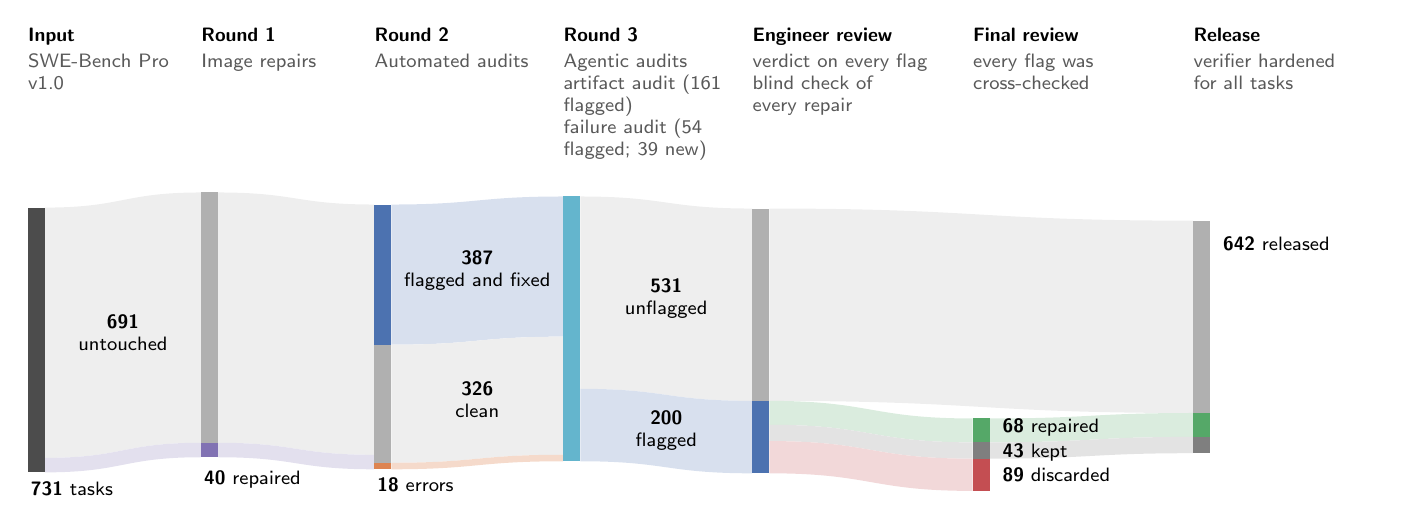
\begin{tikzpicture}[x=1mm, y=1mm, font=\sffamily\scriptsize,
  execute at begin node={\hyphenpenalty=10000\exhyphenpenalty=10000}]
% ---------------------------------------------------------------- bands
% Input -> Round 1: untouched / image repairs
\fill[sbpNone!22] (2.2,-1.92) .. controls (12.1,-1.92) and (12.1,0) .. (22,0)
  -- (22,-31.786) .. controls (12.1,-31.786) and (12.1,-33.706) .. (2.2,-33.706) -- cycle;
\fill[sbpImg!22] (2.2,-33.706) .. controls (12.1,-33.706) and (12.1,-31.786) .. (22,-31.786)
  -- (22,-33.626) .. controls (12.1,-33.626) and (12.1,-35.546) .. (2.2,-35.546) -- cycle;
% Round 1 -> Round 2
\fill[sbpNone!22] (24.2,0) .. controls (34.1,0) and (34.1,-1.53) .. (44,-1.53)
  -- (44,-33.316) .. controls (34.1,-33.316) and (34.1,-31.786) .. (24.2,-31.786) -- cycle;
\fill[sbpImg!22] (24.2,-31.786) .. controls (34.1,-31.786) and (34.1,-33.316) .. (44,-33.316)
  -- (44,-35.156) .. controls (34.1,-35.156) and (34.1,-33.626) .. (24.2,-33.626) -- cycle;
% Round 2 -> Result: flagged / clean / audit errors
\fill[sbpFlag!22] (46.2,-1.53) .. controls (57.1,-1.53) and (57.1,-0.51) .. (68,-0.51)
  -- (68,-18.312) .. controls (57.1,-18.312) and (57.1,-19.332) .. (46.2,-19.332) -- cycle;
\fill[sbpNone!22] (46.2,-19.332) .. controls (57.1,-19.332) and (57.1,-18.312) .. (68,-18.312)
  -- (68,-33.308) .. controls (57.1,-33.308) and (57.1,-34.328) .. (46.2,-34.328) -- cycle;
\fill[sbpErr!30] (46.2,-34.328) .. controls (57.1,-34.328) and (57.1,-33.308) .. (68,-33.308)
  -- (68,-34.136) .. controls (57.1,-34.136) and (57.1,-35.156) .. (46.2,-35.156) -- cycle;
% Result -> Round 3: unflagged / flagged
\fill[sbpNone!22] (70.2,-0.51) .. controls (81.1,-0.51) and (81.1,-2.04) .. (92,-2.04)
  -- (92,-26.466) .. controls (81.1,-26.466) and (81.1,-24.936) .. (70.2,-24.936) -- cycle;
\fill[sbpFlag!22] (70.2,-24.936) .. controls (81.1,-24.936) and (81.1,-26.466) .. (92,-26.466)
  -- (92,-35.666) .. controls (81.1,-35.666) and (81.1,-34.136) .. (70.2,-34.136) -- cycle;
% Round 3 -> Release: never flagged, bypasses engineer review
\fill[sbpNone!22] (94.2,-2.04) .. controls (121.1,-2.04) and (121.1,-3.58) .. (148,-3.58)
  -- (148,-28.006) .. controls (121.1,-28.006) and (121.1,-26.466) .. (94.2,-26.466) -- cycle;
% Round 3 -> Engineer review: repaired / kept / discarded
\fill[sbpRep!22] (94.2,-26.466) .. controls (107.1,-26.466) and (107.1,-28.7) .. (120,-28.7)
  -- (120,-31.736) .. controls (107.1,-31.736) and (107.1,-29.502) .. (94.2,-29.502) -- cycle;
\fill[sbpKeep!22] (94.2,-29.502) .. controls (107.1,-29.502) and (107.1,-31.736) .. (120,-31.736)
  -- (120,-33.806) .. controls (107.1,-33.806) and (107.1,-31.572) .. (94.2,-31.572) -- cycle;
\fill[sbpDisc!22] (94.2,-31.572) .. controls (107.1,-31.572) and (107.1,-33.806) .. (120,-33.806)
  -- (120,-37.9) .. controls (107.1,-37.9) and (107.1,-35.666) .. (94.2,-35.666) -- cycle;
% Engineer review -> Release
\fill[sbpRep!22] (122.2,-28.7) .. controls (135.1,-28.7) and (135.1,-28.006) .. (148,-28.006)
  -- (148,-31.042) .. controls (135.1,-31.042) and (135.1,-31.736) .. (122.2,-31.736) -- cycle;
\fill[sbpKeep!22] (122.2,-31.736) .. controls (135.1,-31.736) and (135.1,-31.042) .. (148,-31.042)
  -- (148,-33.112) .. controls (135.1,-33.112) and (135.1,-33.806) .. (122.2,-33.806) -- cycle;
% ---------------------------------------------------------------- nodes
\fill[black!70] (0,-35.546) rectangle (2.2,-1.92);
\fill[sbpNone]  (22,-31.786) rectangle (24.2,0);
\fill[sbpImg]   (22,-33.626) rectangle (24.2,-31.786);
\fill[sbpFlag]  (44,-19.332) rectangle (46.2,-1.53);
\fill[sbpNone]  (44,-34.328) rectangle (46.2,-19.332);
\fill[sbpErr]   (44,-35.156) rectangle (46.2,-34.328);
\fill[sbpRes]   (68,-34.136) rectangle (70.2,-0.51);
\fill[sbpNone]  (92,-26.466) rectangle (94.2,-2.04);
\fill[sbpFlag]  (92,-35.666) rectangle (94.2,-26.466);
\fill[sbpRep]   (120,-31.736) rectangle (122.2,-28.7);
\fill[sbpKeep]  (120,-33.806) rectangle (122.2,-31.736);
\fill[sbpDisc]  (120,-37.9) rectangle (122.2,-33.806);
\fill[sbpNone]  (148,-28.006) rectangle (150.2,-3.58);
\fill[sbpRep]   (148,-31.042) rectangle (150.2,-28.006);
\fill[sbpKeep]  (148,-33.112) rectangle (150.2,-31.042);
% ---------------------------------------------------------------- labels
\node[anchor=north west, inner sep=1pt] at (0,-36.3) {\textbf{731} tasks};
\node[align=center] at (12.1,-17.8) {\textbf{691}\\untouched};
\node[anchor=north west, inner sep=1pt] at (22,-35.0) {\textbf{40} repaired};
\node[align=center] at (57.1,-9.9) {\textbf{387}\\flagged and fixed};
\node[align=center] at (57.1,-26.3) {\textbf{326}\\clean};
\node[anchor=north west, inner sep=1pt] at (44,-35.8) {\textbf{18} errors};
\node[align=center] at (81.1,-13.5) {\textbf{531}\\unflagged};
\node[align=center] at (81.1,-30.3) {\textbf{200}\\flagged};
\node[anchor=west, inner sep=1pt] at (123.4,-29.9) {\textbf{68} repaired};
\node[anchor=west, inner sep=1pt] at (123.4,-33.0) {\textbf{43} kept};
\node[anchor=west, inner sep=1pt] at (123.4,-35.9) {\textbf{89} discarded};
\node[anchor=west, inner sep=1pt] at (151.4,-6.5) {\textbf{642} released};
% ---------------------------------------------------------------- stage headers
\node[anchor=north west, inner sep=0pt, text width=20mm, align=left] at (0,21)
  {{\bfseries Input}\\[1.5pt]\textcolor{black!65}{SWE-Bench Pro\\v1.0}};
\node[anchor=north west, inner sep=0pt, text width=20mm, align=left] at (22,21)
  {{\bfseries Round 1}\\[1.5pt]\textcolor{black!65}{Image repairs}};
\node[anchor=north west, inner sep=0pt, text width=22mm, align=left] at (44,21)
  {{\bfseries Round 2}\\[1.5pt]\textcolor{black!65}{Automated audits}};
\node[anchor=north west, inner sep=0pt, text width=22mm, align=left] at (68,21)
  {{\bfseries Round 3}\\[1.5pt]\textcolor{black!65}{Agentic audits\\artifact audit (161 flagged)\\failure audit (54 flagged; 39 new)}};
\node[anchor=north west, inner sep=0pt, text width=26mm, align=left] at (92,21)
  {{\bfseries Engineer review}\\[1.5pt]\textcolor{black!65}{verdict on every flag\\blind check of\\every repair}};
\node[anchor=north west, inner sep=0pt, text width=26mm, align=left] at (120,21)
  {{\bfseries Final review}\\[1.5pt]\textcolor{black!65}{every flag was\\cross-checked}};
\node[anchor=north west, inner sep=0pt, text width=24mm, align=left] at (148,21)
  {{\bfseries Release}\\[1.5pt]\textcolor{black!65}{verifier hardened\\for all tasks}};
\end{tikzpicture}}%
\caption{Flow of the 731 tasks from SWE-Bench Pro v1.0 to the released set;
bar and band heights are proportional to task counts. Round~1 repairs 40
container images (leaked test and fixture files, non-standard instructions).
Round~2's automated audit flags 387 tasks (all fixed by human experts). In Round~3, the artifact audit (an LLM agent and a human
auditor compare the instruction with the tests and reference patch) and the
failure audit (an LLM judge attributes failed runs of four agent setups) flag
200 tasks. Engineers adjudicate every flag, and a repair ships only after a
blind re-implementation of the edited instruction passes the hidden tests.}
\label{fig:pipeline}
\end{figure*}

\subsection{Agentic audits}
\label{sec:audits}

\paragraph{Artifact audit.}
An LLM agent compared each task's instruction with its test lists and reference patch, statically without execution. It flagged six patterns: test requirements missing from the instruction, instruction statements contradicted by the tests, test or solution detail copied into the instruction, changed behaviour that no graded test exercises, fixtures read by the tests but never created, and graded lists naming a whole test file. Overly verbose requirement sections were a leakage signal, as they often transcribed the reference patch. An expert human auditor reviewed the agent's flags, and marked high-priority cases. The final audit flagged 161 tasks. 

\paragraph{Failure audit.}
We ran four agent configurations on every task: Claude Code with Claude Opus~5, Codex with GPT-5.6, and mini-SWE-agent with both models. For each run, an LLM judge read the trajectory, patch, verifier log and graded tests and attributes each failure to the model or to the task. A task was flagged when a patch consistent with a reasonable reading of the instruction was rejected. For example, in a \textit{vuls} task two configurations fell back to the bundle directory name as instructed and reported \texttt{Sample.app}, while the graded test expects \texttt{Sample} because the reference patch strips the suffix without the instruction saying so. For each such flag we record the defect type, the fix location, an effort estimate, a proposed edit, and the passing and failing configurations.


\subsection{Defect taxonomy}
\label{sec:taxonomy}

We found six categories of defects, across the instances Table~\ref{tab:repairs-discards}. Unstated requirements, contradictions and verifier/environment defects make correct solutions fail. Leakage and insufficient tests make a task easier than intended or let an incomplete solution pass. 

\begin{table}[t]
\centering
\small
\setlength{\tabcolsep}{3pt}
\begin{tabularx}{\columnwidth}{@{}>{\raggedright\arraybackslash}p{2.05cm} >{\raggedright\arraybackslash}X r r@{}}
\toprule
\textbf{Category} & \textbf{Description} & \textbf{Rep.} & \textbf{Disc.} \\
\midrule
Solution leakage & The instruction gives away test or solution detail. & 18 & 4 \\
\addlinespace
Spec--test contradiction & The instruction contradicts what the tests check. & 10 & 5 \\
\addlinespace
Unstated test requirement & The tests require behaviour, names or files the instruction never states. & 119 & 22 \\
\addlinespace
Insufficient tests & The tests miss part of the change or check incidental details instead of behaviour. & 1 & 33 \\
\addlinespace
Verifier or environment defect & The grading setup or container decides the score regardless of the solution. & 228 & 19 \\
\addlinespace
Miscellaneous & -- & 15 & 6 \\
\midrule
\textbf{Total} & & \textbf{391} & \textbf{89} \\
\bottomrule
\end{tabularx}
\caption{Defect categories of tasks repaired and kept (Rep.) and discarded (Disc.) between the 731 tasks of SWE-Bench Pro Public v1.0 and the final 642. Repairs edited the instruction in 63 tasks and the test patch in 4 (one task both).} %\jeff{Can we clarify that we had more tasks edited than this? Comparing v1.1 and v2.4, instructions are different on 227 tasks. In addition, we edit many verifiers and tasks were also edited between v1 and v1.1. We want to be careful to not make it seem like we are only repairing ~10\% of the tasks}} 
\label{tab:repairs-discards}
\end{table}

%% Needs: \usepackage{booktabs,tabularx}
\begin{table}[t]
\centering\footnotesize
\setlength{\tabcolsep}{3pt}
\begin{tabularx}{\columnwidth}{@{}>{\raggedright\arraybackslash}p{2.05cm}>{\raggedright\arraybackslash}X>{\raggedright\arraybackslash}X@{}}
\toprule
\textbf{Problem} & \textbf{Evidence} & \textbf{Fix} \\
\midrule
\multicolumn{3}{@{}l}{\textit{Data}} \\
Instruction and tests disagree & 94 tasks (Table~\ref{tab:repairs-discards}) & 63 instructions edited; 31 tasks discarded \\
\addlinespace[1.5pt]
Tests too weak & 36 tasks & 3 assertions added; 33 tasks discarded \\
\addlinespace[1.5pt]
Grading or image broken & 19 tasks; shared defects in 253 Go, 322 Python and 47 jest verifiers & 19 tasks discarded; verifiers scoped, capped, re-parsed \\
\addlinespace[1.5pt]
Parser renamed graded tests & Reference patch failed on 23 tasks & Graded names regenerated \\
\addlinespace[1.5pt]
Agent files reach grading & 44 runs zeroed; stale bytecode & Test files, test data and bytecode reset before grading \\
\midrule
\multicolumn{3}{@{}l}{\textit{Evaluation}} \\
Open internet & 32/642 runs reached code hosts; 25 fetched their own repository & Only the model endpoint reachable; probed before each run \\
\addlinespace[1.5pt]
Web tools outside the sandbox & 13/642 runs used web fetch & Disabled \\
\addlinespace[1.5pt]
Grading in the agent's sandbox & A \texttt{python3} wrapper scores an empty patch 1 & Re-graded in a clean container \\
\addlinespace[1.5pt]
Fix in git history & 642 images checked & Fixing commit absent; probed \\
\bottomrule
\end{tabularx}
\caption{Problems found in SWE-Bench Pro and the v2 fix. Data problems concern the tasks; evaluation problems concern how runs are executed and graded.}
\label{tab:problems}
\end{table}

\paragraph{Unstated test requirement (119 repaired, 22 discarded).}
The tests depend on behaviour, names or files the instruction does not mention. For example: the \textit{vuls} bundle-name task mentioned before , was repaired by stating that the \texttt{.app} suffix is removed. We repaired a task when the missing requirement is behaviour the task is about, and discarded it when the test checks how the reference patch happens to be written, since stating that would give the solution away. %Discarded tests read a private attribute (\texttt{\_vmap} in \textit{qutebrowser}), pin avatar CSS classes in a snapshot (element-web), or inspect a private client through \texttt{reflect} and \texttt{unsafe} (flipt). 

\paragraph{Spec--test contradiction (10 repaired, 5 discarded).}
Contradictions whose fix lies in the tests were discarded, for example a \textit{webclients} task whose interface declares an \texttt{Element} argument while the graded test passes a \texttt{Document}.

\paragraph{Solution leakage (18 repaired, 4 discarded).}
Leaky instructions walked through the reference patch file by file, or copied expected values from the tests. Example: a \textit{tutanota} instruction told the agent to update the try-catch block around \texttt{aes256Decrypt} in \texttt{decrypt}. The repaired version specifies behaviour only: a \texttt{CryptoError} raised by the crypto library must surface as the application's own \texttt{CryptoError}, which the credentials layer converts to \texttt{KeyPermanentlyInvalidatedError}. Repairs delete the leaked text and, where a test depends on it, restate the requirement as behaviour. 

\paragraph{Insufficient tests (1 repaired, 33 discarded).}
The graded tests leave part of the change unchecked, for example, in a \textit{flipt} task they cover only the error paths of a new cache layer, so a \texttt{getJSON} that always returns false and a no-op \texttt{setJSON} pass. Engineers did not write new tests, so most of these tasks were discarded. 

\paragraph{Verifier or environment defect (228 repaired, 19 discarded).}
In 16 tasks the fail-to-pass list names a whole file (e.g.\ \texttt{test/tests/calendar/\allowbreak CalendarUtilsTest.js \textbar{} test suite}), so any unrelated or flaky failure in that file fails a correct patch. In 3 tasks the image has issues that prevent grading, for example, a teleport test is skipped because SoftHSM is missing, which the verifier scores as a failure. These tasks needed per-task changes to the graded list or the image, and shared verifier defects were fixed globally (\S\ref{sec:verifier}).


% \subsection{Engineer review}
% \label{sec:review}

\subsection{Engineer review}
\label{sec:review}

Engineers applied one criterion: if the reference patch adds a behaviour and a hidden test checks it, the instruction must state the behaviour, but not how the reference patch implements it. Hidden tests were never edited to agree with an instruction, and instructions were never rewritten to match a wrong test.

23 contracted engineers adjudicated every flag, spending 404 hours in total. For each claim in a flag they recorded whether it holds, holds in part or does not hold, citing evidence by artifact and line (e.g.\ \texttt{requirements:19}, \texttt{golden:562}). A false flag leaves the task unchanged; a gap in the instruction leads to an edit limited to where the flag holds; a remedy that lies in the tests, fixtures, verifier or image leads to quarantine, i.e.\ removal. High-priority flags received a second independent review and a third pass by the project team.

Of the 147 artifact-audit flags, reviewers confirmed 70, partly confirmed 21 and rejected 56: 33 tasks were repaired, 43 kept and 70 discarded. Of the 54 failure-audit flags, 35 were repaired and 19 discarded. The judge's fix location predicted the outcome: 28 of the 31 flags it placed in the instruction were repaired, and 16 of the 23 placed elsewhere were discarded. In all, 68 of the 200 flagged tasks were repaired, 43 kept and 89 discarded (Figure~\ref{fig:pipeline}).
% CHECK: Figure 2 says the artifact audit flagged 161; 147 here must be explained (e.g. 161 minus the 14 second-batch removals) or made to match. Also 33+43+70 = 146, so one of the 147 must be counted under the failure audit.

Repairs were validated blind: a second engineer who had seen neither the original task nor the reference patch implemented the edited instruction, and the edit shipped only if that implementation passed the hidden tests; for the auditors' repairs, the reference patch was re-run against the edited tests. Fourteen tasks repaired in a second batch were removed before release and are counted as discards under their original flag (they include all four leakage discards), and two auditor repairs not carried into the release are counted as kept. Figure~\ref{fig:pipeline} counts a task as repaired when its instruction or test patch changed in response to a flag; Table~\ref{tab:repairs-discards} also counts the final review's task-specific edits.


\subsection{Verifier hardening}
\label{sec:verifier}

Defects in shared grading code were fixed for all tasks.

\paragraph{Scoping and resources.}
The Go verifier ran \texttt{go test ./...} over the whole repository. Scoping it to the graded packages on 253 tasks removed out-of-memory failures and timeouts. Run scripts on 231 tasks that executed the full suite were restricted to the graded tests. With automatic worker counts, pytest-xdist spawned up to 128 workers on small test files and crashed with ``no tests ran'': we capped it at four workers on 239 tasks and inside \texttt{ansible-test} on 83.

\paragraph{Parsing and environment.}
The jest parser assigned tests in failing files to the wrong file and dropped failures (47 tasks), and it truncated test titles at the first parenthesis: it now strips only the trailing timing. We added kernel headers for cgo builds (5 tasks), fetched at grading time one Go module missing from an image's offline cache, re-derived test scoping on 3 tasks that omitted the packages defining the graded tests, and restored CRLF line endings in a fixture that made the reference patch fail.

\paragraph{Test-file reset.}
Before the hidden tests run, the verifier (i)~restores every path the test patch touches and deletes only paths it creates; (ii)~restores modified tracked test data (test data, fixtures, mocks, snapshots), with allowlists for the six reference patches that change fixtures; (iii)~removes agent-written test files that collide with hidden tests; (iv)~clears stale git lock files left by killed agent commands; and (v)~deletes \texttt{\_\_pycache\_\_} and \texttt{.pyc} files. Without (i), agent edits to snapshots owned by the test patch made it fail to apply in 44 runs. Step (v) addresses \texttt{.pyc} files that an agent's \texttt{git stash} round trip left with unchanged size and timestamp, which made the verifier import the base code.

On the assembled 642-task set, the reference patch passes every task and the empty patch fails every task.


\subsection{Hardened evaluation protocol}
\label{sec:protocol}

We run every model under a \textit{locked protocol} where the harness sets network access per phase of a run, and grades the agent's patch in a fresh container rather than in the agent's sandbox. 

\paragraph{Network.}
With the network open, 32 of 642 Claude Opus~5 trajectories contacted code hosts, and 25 downloaded the task's own repository. Under the lock, the sandbox can reach only the model endpoint during the agent phase (the allowlist names that hostname alone) and web tools that scaffolds execute outside the sandbox are disabled.  The git history of all 642 images are scrubbed of the fixing commit.

\paragraph{Grading.}
The original harness ran the verifier in the sandbox the agent had just used. Because the verifier restores test files but not binaries, a scripted agent that edits no source file and replaces \texttt{python3} with a script printing \textsc{PASSED} scores 1. Forged dependencies pass through the same gap: with the network closed, some agents that could not fetch a fix edited the Go module cache in place or served a fabricated module version from a local \texttt{GOPROXY}, and neither change appears in the diff. We now save the agent's changes as a patch, apply it to a fresh copy of the task image, run the unchanged verifier there and report that grade, so that binaries or module caches do not carry over.
%We report both grades for every task. When the two disagree, two more fresh grades decide, by majority.
% CHECK: CHEATING_MODES.md says the fresh re-grade is authoritative and that flips are adjudicated with 2 extra fresh re-grades (a forgery fails 2/2, a flake passes at least 1/2). Align the commented sentence with that before re-enabling it.

\paragraph{Trajectory Audits.}
A fresh re-grade cannot catch a forgery committed inside the patch, so we audit patches for \texttt{replace} directives that point into the patch or to absolute paths, \texttt{go.sum} entries for modules absent from the image, and large new directories that imitate a third-party SDK. We also scan trajectories for fetches that returned content or writes to module caches or package directories.
% CHECK: state whether flagged patches are rejected automatically or reviewed by hand.
